\documentclass{beamer}

% \usetheme{Singapore}
% \usetheme{Malmoe}
\usetheme{Warsaw}

\usepackage[utf8]{inputenc}
\usepackage[russian]{babel}
\usepackage{cmap}
\usepackage{mathrsfs}

% \useoutertheme{split}
\useoutertheme{shadow}
\usefonttheme{professionalfonts}
\usepackage{graphicx}
\usepackage{psfrag}
\beamertemplatenavigationsymbolsempty 
\DeclareMathOperator{\sign}{sign}

\setbeamertemplate{footline}[frame number]

\author{Павел Филонов \\ \href{mailto:filonovpv@gmail.com}{filonovpv@gmail.com}}
\title{Введение в машинное обучение}
\subtitle{Основные понятия и определения}

\begin{document}
\begin{frame}[plain]
    \titlepage
\end{frame}
\begin{frame}[plain]{Содержание}
  \tableofcontents
\end{frame}
\section{Основные понятия и обозначения}
\subsection{Постановка задачи машинного обучения}
\begin{frame}{Постановка задачи машинного обучения}
Пусть
    \begin{itemize}
        \item $X$ --- множество объектов (objects);
        \item $Y$ --- множество ответов (targets);
        \item $y: X \rightarrow Y$ --- неизвестная зависимость (target function).
    \end{itemize}
    {\bf Дано:}
    \begin{itemize}
        \item $\{x_1, \dots, x_l\} \subset X$ --- обучающая выборка (training sample);
        \item $y_i = y(x_i),~ i=1,\dots, \ell$ --- известные ответы (known targets).
    \end{itemize}
    {\bf Найти:}
    $a: X \rightarrow Y$ --- алгоритм, решающую функцию (decision function), приближающую $y$ на всём множестве $X$.


Весь курс машинного обучения--- это конкретизация:
    \begin{itemize}
        \item как задаются объекты и какими могут быть ответы;
        \item в каком смысле <<$a$ приближает $y$>>;
        \item как строить функцию $a$.
    \end{itemize}

% Приведенная задача --- представляет собой центральную проблему, которая красной нитью проходит через весь курс.
\end{frame}

\subsection{Представление объектов и ответов.}
\begin{frame}
$f_j: X \rightarrow D_j, j=1,\dots,n$ --- принаки объектов (features).

Типы признаков:
\begin{itemize}
    \item $D_j = \{0, 1\}$ --- бинарный признак;
    \item $|D_j| < \infty$ --- номинальный признак;
    \item $|D_j| < \infty, ~ D_j - \text{упорядочено}$ --- порядковый признак;
    \item $D_j = \mathbb{R}$ --- количественный признак.
\end{itemize}

Вектор $\left(f_1(x),\dots,f_n(x)\right)$ --- признаковое описание объекта $x$.

Матрица <<объекты-признаки>> (feature matrix)
$$
F = ||f_j(x_i)||_{\ell \times n} = \begin{pmatrix}
    f_1(x_1) & \cdots & f_n(x_1) \\
    \vdots   & \ddots &   \vdots \\
    f_1(x_\ell) & \cdots & f_n(x_\ell) \\
    \end{pmatrix}
$$
\end{frame}

\begin{frame}{Представление ответов. Типы задач}
    
    {\bf Задача классификации} (classification):
    \begin{itemize}
        \item $Y = \{-1, +1\}$ --- бинарная классификация;
        \item $Y = \{1, \dots, M\}$ --- на $M$ непересекающихся классов;
        \item $Y = \{0, 1\}^M$ --- на $M$ классов, которые могут пересекаться.
    \end{itemize}
    \vfill

    {\bf Задача восстановления регресии} (regression):
    \begin{itemize}
        \item $Y = \mathbb{R}$ --- одномерная;
        \item $Y = \mathbb{R}^m, ~ m > 1$ --- многомерная (multivariate).
    \end{itemize}
    \vfill

    {\bf Задача ранжирования} (ranking)
    \begin{itemize}
        \item $Y$ --- конечное упорядоченное множество.
    \end{itemize}
\end{frame}
\begin{frame}{Задача классификации цветков ириса [Фишер, 1936]}
    \footnotesize $n = 4$ количественный признака, $|Y| = 3$ класса, объем выборки $\ell = 150$.
    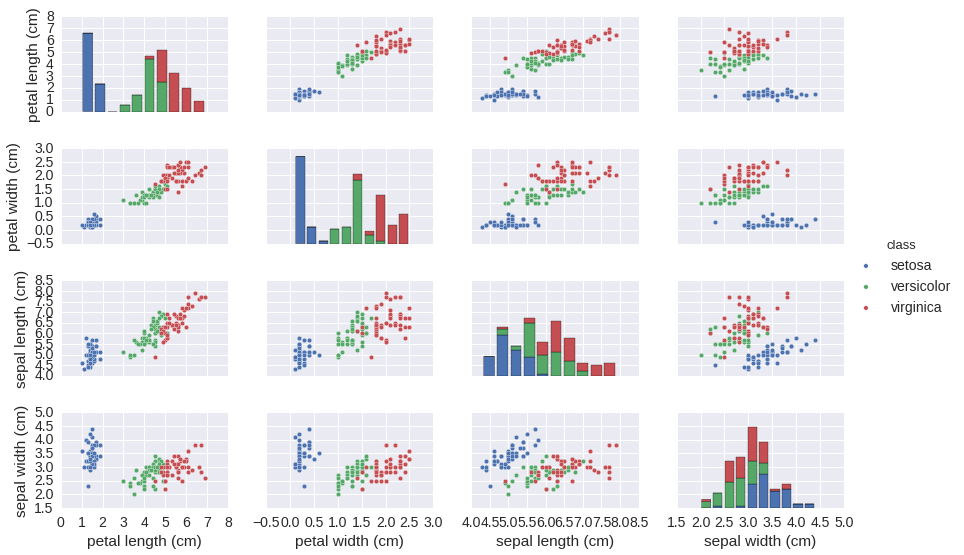
\includegraphics[width=\linewidth]{fig/iris.png}
\end{frame}
\begin{frame}{Задача оценки стоимости жилья в Бостоне}
    \begin{center}
        $n = 13, Y= \mathbb{R}, l = 506$
        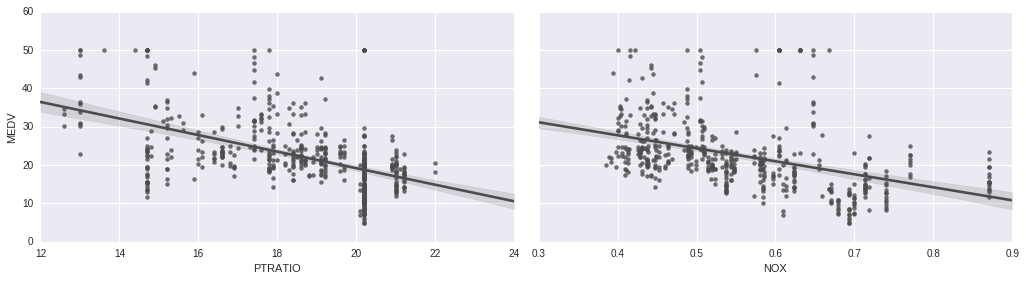
\includegraphics[width=\linewidth]{fig/boston1.png}
        \\
        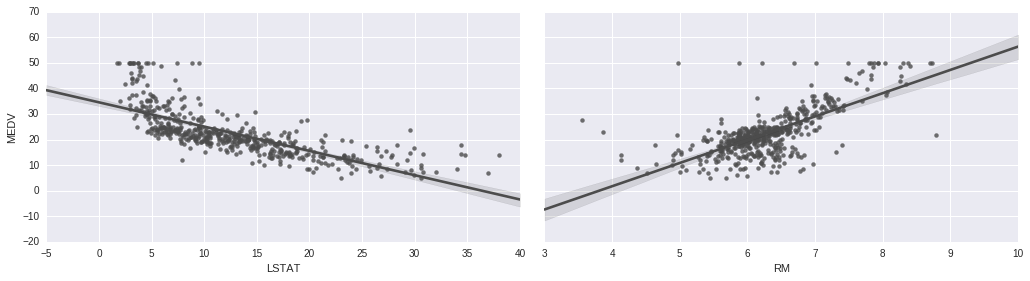
\includegraphics[width=\linewidth]{fig/boston2.png}
    \end{center} 
\end{frame}

\subsection{Модели и методы обучения}
\begin{frame}{Модель алгоритмов}
Модель (predictive model) --- парметрическое семейство функций
$$
    A = \{g(x, \theta) ~|~ \theta \in \Theta\},
$$
где $g : X \times \Theta \rightarrow Y$ --- фиксированная функция,\\
$\Theta$ --- множество допустимых значений параметра $\theta$.

{\bf Пример.}
Линейная модель с вектором параметров $\theta = (\theta_1,\dots,\theta_n), \Theta = \mathbb{R}^n$:
$$
    g(x, \theta) = \sum\limits_{j=1}^{n}\theta_j f_j(x) \text{--- для регресии и ранжирования, $Y = \mathbb{R}$};
$$
$$
    g(x, \theta) = \sign\sum\limits_{j=1}^{n}\theta_j f_j(x) \text{--- для классификации, $Y = \{-1, +1\}$}.
$$
\end{frame}

\begin{frame}{Метод обучения}
Метод обучения (learning algorithm) --- это отображение вида
$$
\mu: (X \times Y)^l \rightarrow A,
$$
которое произвольной выборке $S = (x_i, y_i)_{i=1}^{\ell} \subset (X \times Y)^\ell$ ставит в соответсвие некоторый алгоритм $a \in A$.

В задачах обучения по прецедентам всегда есть два этапа:
\begin{itemize}
    \item Этап обучения (training): \\
    метод $\mu$ по выборке $S$ строит алгоритм $a = \mu(S)$.
    \item Этап применеия (testing): \\
    алгоритм $a$ для новых объектов $x \in X$ выбаёт ответы $a(x) \in Y$.

\end{itemize}
\end{frame}

\subsection{Обучение и переобучение}
\begin{frame}{Функционалы качества}
$\mathscr{L}(a, x, y)$ --- функция потерь (loss function) --- величина ошибки алгоритма $a \in A$ на объекте $x \in X$.

{\bf Функции потерь для задач классификации:}
\begin{itemize}
    \item $\mathscr{L}(a, x, y) = [a(x) \ne y(x)]$ --- индикатор ошибки.
\end{itemize}

{\bf Функции потерь для задач регрессии:}
\begin{itemize}
    \item $\mathscr{L}(a, x, y) = |a(x) - y(x)|$ --- абсолютное значение ошибки;
    \item $\mathscr{L}(a, x, y) = \left(a(x) - y(x)\right)^2$ --- квадратичная ошибка.
\end{itemize}

{\it Эмпирический риск} --- функционал качества алгоритма $а$ на $S = \{(x_i, y_i)\}_{i=1}^{\ell}$:
$$
Q(a, S) = \frac{1}{\ell}\sum\limits_{i = 1}^{\ell}\mathscr{L}(a, x_i, y_i).
$$
\end{frame}

\begin{frame}{Сведение задачи обучения к задача оптимизации}
Метод минимизации эмпирического риска:
$$
\mu(S) = \arg\min_{a \in A} Q(a, S)
$$

{\bf Пример:} метод наименьших квадратов ($Y = \mathbb{R}, \mathscr{L}$ квадратична):
$$
\mu(S) = \arg\min_{theta}\sum\limits_{i=1}{\ell}\left(g(x_i, \theta) - y_i\right)^2.
$$

{\bf Проблемы обобщающей способности:}
\begin{itemize}
    \item найдём ли мы <<закон природы>> или переобучимся (overfitting), т.е. подгоним функцию $g(x_i,\theta)$ под заданные точки?
    \item будет ли $a = \mu(S)$ приближать функцию $y$ на всём $X$?
    \item будет ли $Q(a, S)$ мало на новых данных --- контрольной выборке (validation set) $S' = \{(x_i', y_i')\}_{i=1}^{k}$?
\end{itemize}
\end{frame}

\begin{frame}{Пример переобучения}
Переобучение --- это когда $Q(\mu(S'), S') \gg Q(\mu(S), S)$.

Значения функции потерь для задачи прогноза цены на жилье в Бостоне.
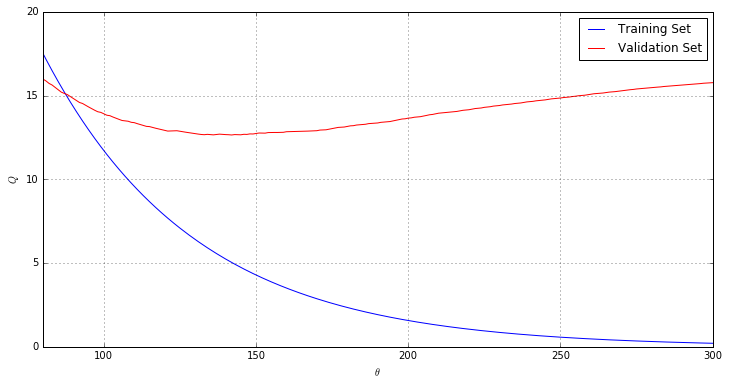
\includegraphics[width=\linewidth]{fig/overfitting.png}
\end{frame}

\begin{frame}{Переобучение --- одна из проблем машинного обучения}
\begin{itemize}
    \item {\bf Из-за чего возниает переобучение?}
    \begin{itemize}
        \item - избыточная сложность пространства параметров $\Theta$, лишние степени свободы в модели $g(x, \theta)$ <<тратятся>> на чрезмерно точную подгонку под обучающую выборку;
        \item переобучение есть всегда, когда есть оптимизация параметров по конечной (заведомо неполной) выборке.
    \end{itemize}
    \item {\bf Как обнаружить переобучение?}
    \begin{itemize}
        \item эмпирически, путём разбиения выборки на обучающую (train) и контрольную (validate, test).
    \end{itemize}
    \item {\bf Избавиться от него нельзя. Как его минимизировать?}
    \begin{itemize}
        \item минимизировать одну из теоретических оценок;
        \item накладывать ограничения на $\theta$ (регуляризация);
        \item минимизировать hold-out, LOO или CV.
    \end{itemize}
\end{itemize}
\end{frame}

\begin{frame}{Эмпирические оценки обобщающей способности}
\begin{itemize}
    \item Эмпирический риск на контрольных данных (hold-out):
    $$
        HO(\mu, S, S') = Q(\mu(S), S') \rightarrow \min
    $$
    \item Скользяший контроль (leave one out):
    $$
        LOO(\mu, S) = \frac{1}{\ell}\sum\limits_{i=1}^{\ell}\mathscr{L}(\mu(S\setminus \{x_i\}), y_i) \rightarrow \min
    $$
    \item Кросс-проверка (cross-validation), $S = T_n \sqcup V_n$
    $$
        CV(\mu, S) = \frac{1}{|N|}\sum\limits_{n \in N} Q(\mu(T_n), V_n) \rightarrow \min
    $$
    \item Эмпирическая оценка вероятности переобучения:
    $$
    Q_{\varepsilon}(\mu, S) = \frac{1}{|N|}\sum\limits_{n \in N}\lbrack Q(\mu(T_n), V_n) - Q(\mu(T_n), T_n) \ge \varepsilon \rbrack \rightarrow \min
    $$
\end{itemize}
\end{frame}
% \begin{frame}{Машинное обучение ранжированию <<Интернет-математика 2009>>}

% \end{frame}
\section{Примеры прикладных задач}
\subsection{Пример 1}
\begin{frame}
\end{frame}
\subsection{Пример 2}
\begin{frame}
\end{frame}
\section{Методология машинного обучения}
\subsection{Межотраслевой стандарт CRISP-DM}
\begin{frame}{\large CRISP-DM: Cross Industry Standard Process for Data Mining}
% Cross Industry Standard Process for Data Mining
\begin{center}
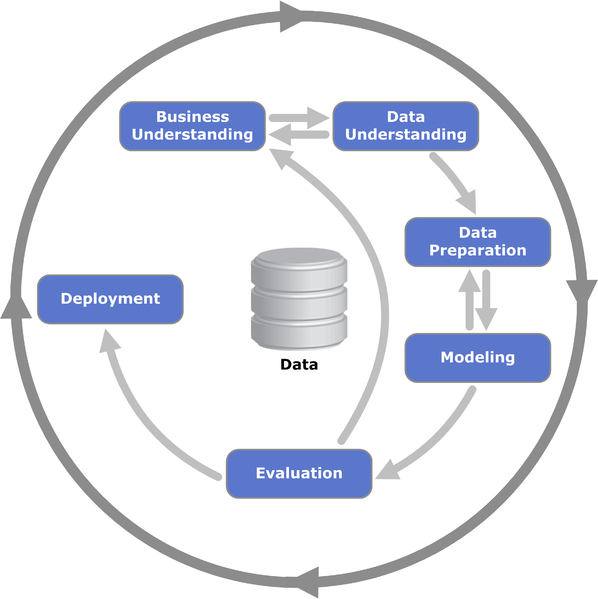
\includegraphics[width=0.68\linewidth]{fig/CRISP-DM.png}
\end{center}
\end{frame}
\end{document}